\section{个性化PageRank}
\label{sec:graph-personalized-pagerank}

上一节的标准PageRank取均匀跳转分布$\bm s=\frac1n\bm 1^\top$，计算出的是所有节点与查询者无关的“全局通用权威分”。如果我们将重启分布$\bm s$集中到某一个指定节点$u$（或少数几个节点）上，让随机游走每次重启时都回到$u$重新出发，所得的平稳分布就称为\term{个性化PageRank}（personalized PageRank，简称PPR），其中的起点称为\term{种子}（seed）。本节按照“背景与主要思想—算法实现—算法分析”的脉络，介绍个性化PageRank及其在超大规模图上的局部推送算法与局部谱划分应用。

\subsection{背景与主要思想}
\label{sec:graph-pagerank-push-principle}

\paragraph{为什么引入个性化PageRank}

全局排名与针对某个种子的关联排名回答不同的问题。将重启分布集中在顶点$u$后，游走反复从$u$出发，短路径的传播权重通常高于长路径。个性化PageRank由图结构、转移概率与重启概率共同确定，因而可作为相对于种子的关联度量；它不等同于最短路距离，也不保证得分高的顶点一定与种子直接相邻。

第二个问题是如何利用稀疏种子进行局部计算。全局幂迭代通常读取整张图，而局部查询未必需要计算每个顶点的精确分数。重启使长度为$t$的传播项按几何因子衰减，但这不自动保证某个小邻域包含绝大多数概率质量。下面的局部推送通过截断单位度数余量，给出显式的工作量与误差界；在参数和种子支撑较小时，它可能只访问图的一部分。

\paragraph{主要思想：种子重启与局部推送（Local Push）}

本节在至少有两个顶点的连通简单无权图上考察采用惰性转移矩阵$\bm Q=(\bm I+\bm P)/2$的个性化PageRank。在个性化PageRank与局部算法文献中，习惯用$\alpha\in(0,1)$直接表示每一步的\emph{重启（或就地终止）概率}，用$1-\alpha$表示沿惰性矩阵$\bm Q$继续游走一步的概率（对应上一节的阻尼系数$1-\alpha$）。对于任意非负种子向量$\bm s\in\mathbb R^{1\times n}$（通常取单点种子$\bm s=\bm e_u^\top$），对应的个性化PageRank线性算子$\mathcal R(\bm s)$定义为
\begin{equation}
\mathcal{R}(\bm{s})
=\alpha\sum_{t=0}^{\infty}(1-\alpha)^t\bm{s}\bm{Q}^t,
\label{eq:graph-pagerank-linear-operator}
\end{equation}
其满足不动点方程$\mathcal R(\bm s)=\alpha\bm s+(1-\alpha)\mathcal R(\bm s)\bm Q$，且对任意待分配质量行向量$\bm r$满足一步分解恒等式：
\begin{equation}
\mathcal{R}(\bm{r})=\alpha\bm{r}+(1-\alpha)\mathcal{R}(\bm{r}\bm{Q}).
\label{eq:graph-pagerank-push-decomposition}
\end{equation}

如何在不扫描全图的前提下算出$\mathcal R(\bm s)$的高精度近似？Andersen、Chung与Lang于2006年提出了著名的\emph{局部推送}（local push，或ApproximatePR）思想\scite{andersen2006localpagerank}。

其核心设计首先在于\emph{维护“已确认分数$\bm p$ + 待处理余量$\bm r$”的质量守恒不变量}。局部推送不像全局幂法那样每轮同步更新全图所有节点，而是维护两个稀疏行向量：一个是记录已经终止游走、已累积的终点分数的\emph{近似向量}$\bm p$，另一个是记录当前仍滞留在各节点等待继续向外扩散的\emph{余量向量}（residual）$\bm r$。初始时令已确认分数$\bm p=\bm 0$，并将全部初始种子质量放入待处理余量$\bm r=\bm s$。

在每一步局部操作中，算法只单独挑出一个节点$i$，将它当前积压的余量$q=r_i$清空，并按一步分解式~\eqref{eq:graph-pagerank-push-decomposition}拆成两部分处理：其中$\alpha q$比例就地停止游走，直接累加到已确认分数$p_i$中；其余$(1-\alpha)q$比例则按惰性矩阵$\bm Q$向前推进一步，分发给节点$i$自身及它的直接邻居作为新的待处理余量。

由于每次推送只是把单个节点$i$的待处理质量沿着随机游走规则向前推进了一步，整个算法运行期间始终严格保持如下质量守恒不变量：
\begin{equation}
\mathcal{R}(\bm{s})=\bm{p}+\mathcal{R}(\bm{r}).
\label{eq:graph-pagerank-push-invariant}
\end{equation}

对顶点$i$推送一次需读取$d_i$个邻居。用阈值$r_i/d_i>\varepsilon$筛选活跃顶点，便能将每次读取的邻接表大小与被转移到$\bm p$中的质量联系起来。当所有余量均满足$r_i\leq\varepsilon d_i$时停止，可得到逐点误差界。算法不必展开所有顶点的邻接表，但仍会读取被推送顶点的邻居标识并更新余量；是否为亚线性工作量取决于$\alpha,\varepsilon$和种子支撑。

\subsection{算法实现}
\label{sec:graph-pagerank-push-implementation}

\paragraph{局部推送算法步骤}

在简单无权图上，惰性转移矩阵$\bm Q=(\bm I+\bm P)/2$将一半质量留在当前顶点$i$，另一半质量均分给$i$的$d_i$个邻居。因此，对顶点$i$（旧余量记为$q=r_i$）执行一次局部推送的更新公式为
\begin{equation}
\begin{aligned}
p_i &\leftarrow p_i+\alpha q,\\
r_i &\leftarrow (1-\alpha)q/2,\\
r_j &\leftarrow r_j+(1-\alpha)q/(2d_i),\qquad \forall j\sim i.
\end{aligned}
\label{eq:graph-pagerank-push-update}
\end{equation}
采用哈希表（字典）稀疏存储$\bm p$与$\bm r$，并用队列维护满足$r_i>\varepsilon d_i$的活跃顶点，完整算法如下。

\begin{algorithm}[个性化PageRank局部推送（Local Push）]
\label{alg:graph-personalized-pagerank-push}
输入：可按点查询且能常数时间读取度数的无向图邻接表、稀疏种子分布$\bm{s}$、重启概率$\alpha\in(0,1)$、截断阈值$\varepsilon>0$。输出：稀疏近似分数$\bm{p}$与剩余余量$\bm{r}$。
\begin{enumerate}
  \item \textbf{稀疏初始化}：令$\bm{p}=\bm{0}$、$\bm{r}=\bm{s}$。将所有满足$r_i>\varepsilon d_i$的顶点$i$加入活跃队列$Q$。
  \item \textbf{局部推送循环}：当队列$Q$非空时，弹出队首顶点$i$，记其当前余量为$q=r_i$，按式~\eqref{eq:graph-pagerank-push-update}执行局部推送：
    \begin{enumerate}
    \item 划入已确认分数：$p_i\leftarrow p_i+\alpha q$；
    \item 更新本点惰性停留余量：$r_i\leftarrow(1-\alpha)q/2$；
    \item 分发邻居余量：遍历$i$的每个邻居$j\sim i$，令$r_j\leftarrow r_j+(1-\alpha)q/(2d_i)$。
    \end{enumerate}
    更新完毕后，检查顶点$i$及每个邻居$j\sim i$：若某个顶点满足$r_v>\varepsilon d_v$且不在队列$Q$中，将其加入队尾。
  \item \textbf{终止返回}：当队列$Q$为空时停止，返回稀疏向量$\bm{p}$和$\bm{r}$。
\end{enumerate}
\end{algorithm}

\paragraph{四点路径上的三次推送演示}

在单位权四点路径$1\!-\!2\!-\!3\!-\!4$上取单点种子$1$（$\bm s=(1,0,0,0)$），重启概率$\alpha=1/2$，阈值$\varepsilon=1/8$。四个顶点的度依次为$1,2,2,1$，对应的触发阈值$\varepsilon d_i$依次为$\frac18,\frac14,\frac14,\frac18$。
\begin{itemize}
\item \emph{第一次推送顶点$1$}：旧余量$q=1>\frac18$。划入分数$p_1\leftarrow\frac12$；剩余$\frac12$对半分，$r_1\leftarrow\frac14$留在本点，$r_2\leftarrow\frac14$送给邻居$2$，此时$\bm p=(\frac12,0,0,0),\bm r=(\frac14,\frac14,0,0)$。因$r_1=\frac14>\frac18$仍超阈值，顶点$1$继续留在队列中（而$r_2=\frac14$未严格超过$\varepsilon d_2=\frac14$）。
\item \emph{第二次推送顶点$1$}：旧余量$q=\frac14$。划入分数$\frac18$使$p_1=\frac58$；剩余$\frac18$对半分，$r_1\leftarrow\frac{1}{16}$，$r_2\leftarrow\frac14+\frac{1}{16}=\frac{5}{16}$。此时$\bm p=(\frac58,0,0,0),\bm r=(\frac{1}{16},\frac{5}{16},0,0)$，顶点$2$的余量$\frac{5}{16}>\frac14$超过阈值，进入队列。
\item \emph{第三次推送顶点$2$}（图~\ref{fig:graph-pagerank-third-push}）：旧余量$q=\frac{5}{16}$。划入分数$p_2\leftarrow\frac{5}{32}$；剩余$\frac{5}{32}$中一半$\frac{5}{64}$留作$r_2$，另一半$\frac{5}{64}$均分给邻居$1$和$3$（各加$\frac{5}{128}$）。合并后得到
\[
\bm{p}=\left(\frac58,\frac{5}{32},0,0\right),\qquad
\bm{r}=\left(\frac{13}{128},\frac{5}{64},\frac{5}{128},0\right).
\]
此时四个顶点的余量均不再超过各自阈值$\frac18,\frac14,\frac14,\frac18$，队列为空，算法终止。注意最右端的顶点$4$在整个运行过程中从未被访问过（$p_4=r_4=0$）。图~\ref{fig:pagerank-push-evolution}以柱状图直观展示了三次推送中$\bm p$与$\bm r$的消长过程。
\end{itemize}

\begin{BookInlineFigure}
\centering
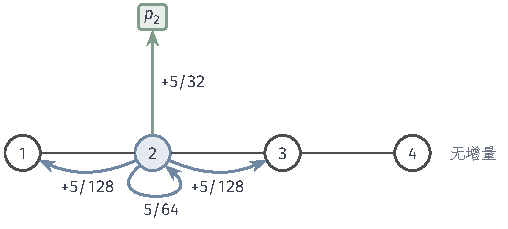
\includegraphics[width=85.965mm]{figures/03-graphs/05-matrices-and-spectra/tikz/walk-examples/pagerank-push-path.pdf}
\caption{四顶点路径上的第三次局部推送（$\alpha=1/2$）。从顶点$2$取出旧余量$5/16$：向上箭头将$5/32$确认为终点分数$p_2$，回环将$5/64$留作本点余量，左右箭头向邻居$1,3$各分发$5/128$余量。}
\label{fig:graph-pagerank-third-push}
\end{BookInlineFigure}

\begin{figure}[!htb]
\centering
\begin{tikzpicture}[x=1mm,y=1mm,
  pbar/.style={fill=FigureBlueFill,draw=FigureBlue,line width=.4pt},
  rbar/.style={fill=FigureYellowFill,draw=FigureYellow,line width=.4pt},
  panel/.style={anchor=mid,font=\figurefont\footnotesize},
  vlabel/.style={font=\figurefont\fontsize{6.5}{8}\selectfont,FigureInk,anchor=north},
  plabel/.style={font=\figurefont\fontsize{6}{7.5}\selectfont,FigureInk,anchor=south}]
  \def\bw{2.6}
  \def\sc{32}
  \def\gp{1.2}
  \def\vgp{3.0}
  \fill[pbar] (0,27) rectangle +(3,2); \node[font=\figurefont\fontsize{6.5}{8}\selectfont,anchor=west] at (4,28) {分数$p_i$};
  \fill[rbar] (20,27) rectangle +(3,2); \node[font=\figurefont\fontsize{6.5}{8}\selectfont,anchor=west] at (24,28) {余量$r_i$};
  \begin{scope}[xshift=0mm]
    \draw[FigureStroke,line width=.35pt] (0,0) -- (0,\sc*0.55);
    \draw[FigureStroke,line width=.35pt] (0,0) -- (4*2*\bw+4*\gp+3*\vgp+1,0);
    \foreach \i/\v/\pv/\rv in {0/1/0.5/0.25, 1/2/0/0.25, 2/3/0/0, 3/4/0/0} {
      \pgfmathsetmacro{\x}{\i*(2*\bw+\gp+\vgp)+1}
      \pgfmathsetmacro{\hp}{\pv*\sc}
      \pgfmathsetmacro{\hr}{\rv*\sc}
      \pgfmathparse{\pv>0?1:0}\ifnum\pgfmathresult=1
        \fill[pbar] (\x,0) rectangle +(\bw,\hp);
      \fi
      \pgfmathparse{\rv>0?1:0}\ifnum\pgfmathresult=1
        \fill[rbar] (\x+\bw+\gp,0) rectangle +(\bw,\hr);
      \fi
      \node[vlabel] at (\x+\bw+\gp/2,-1) {$\v$};
    }
    \node[panel] at (15,-7) {(a) 第$1$次推送后};
  \end{scope}
  \begin{scope}[xshift=36mm]
    \draw[FigureStroke,line width=.35pt] (0,0) -- (0,\sc*0.7);
    \draw[FigureStroke,line width=.35pt] (0,0) -- (4*2*\bw+4*\gp+3*\vgp+1,0);
    \foreach \i/\v/\pv/\rv in {0/1/0.625/0.0625, 1/2/0/0.3125, 2/3/0/0, 3/4/0/0} {
      \pgfmathsetmacro{\x}{\i*(2*\bw+\gp+\vgp)+1}
      \pgfmathsetmacro{\hp}{\pv*\sc}
      \pgfmathsetmacro{\hr}{\rv*\sc}
      \pgfmathparse{\pv>0?1:0}\ifnum\pgfmathresult=1
        \fill[pbar] (\x,0) rectangle +(\bw,\hp);
      \fi
      \pgfmathparse{\rv>0?1:0}\ifnum\pgfmathresult=1
        \fill[rbar] (\x+\bw+\gp,0) rectangle +(\bw,\hr);
      \fi
      \node[vlabel] at (\x+\bw+\gp/2,-1) {$\v$};
    }
    \node[panel] at (15,-7) {(b) 第$2$次推送后};
  \end{scope}
  \begin{scope}[xshift=72mm]
    \draw[FigureStroke,line width=.35pt] (0,0) -- (0,\sc*0.7);
    \draw[FigureStroke,line width=.35pt] (0,0) -- (4*2*\bw+4*\gp+3*\vgp+1,0);
    \foreach \i/\v/\pv/\rv in {0/1/0.625/0.1016, 1/2/0.1563/0.0781, 2/3/0/0.0391, 3/4/0/0} {
      \pgfmathsetmacro{\x}{\i*(2*\bw+\gp+\vgp)+1}
      \pgfmathsetmacro{\hp}{\pv*\sc}
      \pgfmathsetmacro{\hr}{\rv*\sc}
      \pgfmathparse{\pv>0?1:0}\ifnum\pgfmathresult=1
        \fill[pbar] (\x,0) rectangle +(\bw,\hp);
      \fi
      \pgfmathparse{\rv>0?1:0}\ifnum\pgfmathresult=1
        \fill[rbar] (\x+\bw+\gp,0) rectangle +(\bw,\hr);
      \fi
      \node[vlabel] at (\x+\bw+\gp/2,-1) {$\v$};
    }
    \node[panel] at (15,-7) {(c) 第$3$次推送后};
  \end{scope}
\end{tikzpicture}
\caption{四点路径上三次局部推送后的已确认分数$\bm{p}$（蓝色）与待处理余量$\bm{r}$（黄色）。每次推送仅在局部更新被推顶点及其邻居，远端顶点$4$始终未被触及。}
\label{fig:pagerank-push-evolution}
\end{figure}

\subsection{算法分析}
\label{sec:graph-pagerank-push-analysis}

下面证明局部推送的邻接表访问总量与逐点误差界。推送部分的工作量为$O(1/(\alpha\varepsilon))$，另需读取并初始化种子向量的非零支撑；该上界不显式含$n,m$，但参数随图规模变化时并不保证亚线性。局部划分的质量还需要额外的种子和参数条件。

\begin{theorem}[局部推送算法的复杂度与逐点误差界]
\label{thm:graph-pagerank-push-guarantee}
设在连通简单无权图上对非负种子行向量$\bm s$（$\lVert\bm s\rVert_1\leq 1$）、重启概率$\alpha\in(0,1)$和阈值$\varepsilon>0$运行算法~\ref{alg:graph-personalized-pagerank-push}。则算法必在有限步内停止，且满足：
\begin{enumerate}
  \item \emph{总工作量与支撑集上界}：整个运行过程中所有推送操作访问的邻接表边数总和（及已确认分数$\bm p$的非零支撑集体积）满足
  \begin{equation}
  \operatorname{vol}\bigl(\operatorname{supp}(\bm p)\bigr)
  \le \sum_{\text{各次推送}\;i}d_i
  \le \frac{\lVert\bm s\rVert_1}{\alpha\varepsilon}
  \le \frac{1}{\alpha\varepsilon}.
  \label{eq:graph-pagerank-push-work}
  \end{equation}
  \item \emph{逐点相对度数误差与总质量守恒}：算法停止时输出的$(\bm p,\bm r)$对全图每个顶点$i\in V$满足
  \begin{equation}
  0\le\mathcal{R}(\bm{s})_i-p_i\le\varepsilon d_i,
  \qquad
  \frac{\mathcal{R}(\bm s)_i}{d_i} - \varepsilon \le \frac{p_i}{d_i} \le \frac{\mathcal{R}(\bm s)_i}{d_i},
  \label{eq:graph-pagerank-push-pointwise}
  \end{equation}
  且$\ell^1$总误差恒等于剩余余量的总质量：
  \begin{equation}
  \lVert\mathcal{R}(\bm{s})-\bm{p}\rVert_1=\lVert\bm{r}\rVert_1.
  \label{eq:graph-pagerank-push-mass}
  \end{equation}
\end{enumerate}
\end{theorem}

\begin{proof}
（1）每次从队列中弹出顶点$i$执行推送时，该点必满足触发条件$q=r_i>\varepsilon d_i$。此次推送将$\alpha q>\alpha\varepsilon d_i$的质量从余量$\bm r$转化为已确认分数$\bm p$，而其余$(1-\alpha)q$的质量只是在余量向量内部重新分配，因此余量总和$\lVert\bm r\rVert_1$在此次推送中净减少$\alpha q>\alpha\varepsilon d_i$。由于初始余量总和为$\lVert\bm s\rVert_1\leq 1$且余量始终非负，全部推送操作累计减少的余量不可能超过$\lVert\bm s\rVert_1$：
\[
  \sum_{\text{各次推送}\;i}\alpha\varepsilon d_i \leq \sum_{\text{各次推送}\;i}\alpha q \leq \lVert\bm s\rVert_1\leq 1.
\]
由于每个顶点的度至少为$1$，每次推送至少减少$\alpha\varepsilon$的余量，因此推送次数有限。两边同除以$\alpha\varepsilon$即得式~\eqref{eq:graph-pagerank-push-work}（每个$p_i>0$的顶点至少被推送过一次，故$\operatorname{vol}(\operatorname{supp}(\bm p))\leq\sum d_i\leq\frac{1}{\alpha\varepsilon}$）。

（2）算法停止时队列为空，说明每个顶点$i\in V$的剩余余量均满足$0\leq r_i\leq\varepsilon d_i$，即逐分量有$\bm 0^\top\leq\bm r\leq\varepsilon\bm d^\top$。在无向图上，由详细平衡知度向量满足$\bm d^\top\bm P=\bm d^\top$，从而在惰性矩阵$\bm Q=(\bm I+\bm P)/2$下同样满足平稳性$\bm d^\top\bm Q=\bm d^\top$。因为$\bm Q$的元素全部非负，右乘$\bm Q^t$保持逐分量不等号方向：
\[
  \bm 0^\top\leq\bm r\bm Q^t\leq\varepsilon\bm d^\top\bm Q^t=\varepsilon\bm d^\top\qquad(\forall t\geq 0).
\]
代入级数定义~\eqref{eq:graph-pagerank-linear-operator}并结合守恒不变量~\eqref{eq:graph-pagerank-push-invariant}的$\mathcal R(\bm s)-\bm p=\mathcal R(\bm r)$，立得
\[
  \bm 0^\top\leq\mathcal R(\bm s)-\bm p=\alpha\sum_{t=0}^\infty(1-\alpha)^t\bm r\bm Q^t\leq\alpha\sum_{t=0}^\infty(1-\alpha)^t\varepsilon\bm d^\top=\varepsilon\bm d^\top,
\]
取第$i$个分量即为式~\eqref{eq:graph-pagerank-push-pointwise}。最后，因$\mathcal R(\bm r)\geq\bm 0^\top$且算子$\mathcal R$保持向量分量和不变，有$\lVert\mathcal R(\bm s)-\bm p\rVert_1=\lVert\mathcal R(\bm r)\rVert_1=\lVert\bm r\rVert_1$。
\end{proof}

\paragraph{基于个性化PageRank的局部谱划分}

定理~\ref{thm:graph-pagerank-push-guarantee}给出的一个结论是式~\eqref{eq:graph-pagerank-push-pointwise}第二式：局部推送得到的单位度数分数$p_i/d_i$是对真实平稳概率比$\mathcal R(\bm s)_i/d_i$的$\varepsilon$一致逼近，且非零支撑集$S_+=\{i\in V:p_i>0\}$的体积至多为$\frac{1}{\alpha\varepsilon}$。

在全图体积已给定的前提下，这使我们能够将第~\ref{chap:spectral-partition}章的阈值扫描搬到种子附近的候选顶点集$S_+$上（割权与体积仍按原图计算，不能丢弃通向$V\setminus S_+$的边）：只需将满足$p_i>0$的少量顶点按归一化分数$p_i/d_i$从大到小排序，依次扫描非空且不等于全图的前缀集合，并选出导通率$\phi(S)$最小的切分（耗时为$O(\frac{1}{\alpha\varepsilon}\log n)$）。

例如在两个三角形$\{1,2,3\}$与$\{4,5,6\}$经桥边$\{3,4\}$相连的杠铃图上，取$\alpha=1/5,\varepsilon=1/25$，从种子$1$出发执行局部推送后仅顶点$1,2,3$获得正分数，按$p_i/d_i$排序扫描出的前缀$\{1,2,3\}$直接命中了导通率$\phi=1/7$的左团瓶颈割。

这一算例不构成对任意种子和参数的质量保证。Andersen、Chung与Lang的局部划分结果还要求种子属于目标集合中的良种子集，并按目标导通率选择重启概率、截断精度及体积尺度\scite{andersen2006localpagerank}。

原文的精确PageRank扫描保证与带体积筛选的PageRank-Nibble算法是不同结果：后者在给定目标导通率$\varphi$和尺度$2^b$时具有$O(2^b\log^3 m/\varphi^2)$的运行时间界，目标集合还须满足相应的导通率与体积条件。不能将其直接归结为本节任意参数下的局部推送保证。
